\documentclass[letterpaper,twocolumn,10pt]{article}
\usepackage{usenix2020_SOUPS} % journal style template

\usepackage{tikz} % for all things floating
\usepackage{amsmath} % math and formulae
\usepackage{subcaption} % subfigures
%\usepackage{verbatim} % block comments
\usepackage{booktabs}
\usepackage{xurl} % clean line breaks in urls (bibliography in particular looks much better)


\usepackage{color}
\definecolor{red}{rgb}{1,0,0}
\definecolor{orange}{rgb}{1,0.7,0}
\definecolor{dkgreen}{rgb}{0,0.6,0}
\newcommand{\todo}[1]{{\color{red}\bf\em TODO: #1}}

\usepackage{filecontents}
\microtypecontext{spacing=nonfrench}
\pagenumbering{gobble} % do not include page numbers

%------------------------------------------------------------------------------
\begin{document}
%-------------------------------------------------------------------------------
% \keywords{Web Privacy, Browser History Fingerprint, Fingerprinting, Replication, Behavioral Tracking}
\date{} % don't want date printed
% make title bold and 14 pt font (Latex default is non-bold, 16 pt)
\title{\Large \bf Replication: Why We Still Can't Browse in Peace: On the Uniqueness and Reidentifiability of Web Browsing Histories}
%
\def\plainauthor{Author name(s) for PDF metadata. Don't forget to anonymize for submission!}
%
\author{
{\rm Sarah Bird}\\
Mozilla
\and
{\rm Ilana Segall}\\
Mozilla
\and
{\rm Martin Lopatka}\\
Mozilla
} % end author
%
\maketitle
\thecopyright
%-------------------------------------------------------------------------------
\begin{abstract}
%-------------------------------------------------------------------------------
We examine the threat to individuals' privacy based on the feasibility of reidentifying users through distinctive profiles of their browsing history visible to websites and third parties.
This work replicates and extends the 2012 paper \textit{Why Johnny Can't Browse in Peace: On the Uniqueness of Web Browsing History Patterns}~\cite{olejnikWhyJohnnyCan2012}. The original work demonstrated that browsing profiles are highly distinctive and stable.
We reproduce those results and extend the original work to detail the privacy risk posed by the aggregation of browsing histories. 
Our dataset consists of two weeks of browsing data from \textasciitilde{52,000} Firefox users.
Our work replicates the original paper's core findings by identifying 48,919 distinct browsing profiles, of which 99\% are unique.
High uniqueness holds even when histories are truncated to just 100 top sites.
We then find that for users who visited 50 or more distinct domains in the two-week data collection period, \textasciitilde{50\%} can be reidentified using the top 10k sites.
Reidentifiability rose to over 80\% for users that browsed 150 or more distinct domains. 
Finally, we observe numerous third parties pervasive enough to gather web histories sufficient to leverage browsing history as an identifier.

\end{abstract}
%-------------------------------------------------------------------------------
\section{Introduction}
%-------------------------------------------------------------------------------
\label{sec:intro}
Web tracking is the process by which parties with visibility into web traffic identify distinctive patterns of navigation in order to attribute browsing history to specific individuals. 
Third-party trackers remain a major concern; their prevalence and mass tracking activity is well documented~\cite{zeberwww2020, 10.1145/3178876.3186097, 8270427}. 
This work seeks to reproduce the findings of Olejnik, Castelluccia, and Janc~\cite{olejnikWhyJohnnyCan2012} regarding the leakage of private information when users browse the web. 
The reach of large-scale providers of analytics and advertisement services into the overall set of web properties shows a continued increase in visibility~\cite{zeberwww2020} by such parties across a plurality of web properties.
This makes the threat of history-based profiling even more tangible and urgent now than when originally proposed.
%
%-------------------------------------------------------------------------------
\section{Background and related work}
%-------------------------------------------------------------------------------
\label{sec:background}
As a replication of prior work, this manuscript presumes some familiarity with the source manuscript~\cite{olejnikWhyJohnnyCan2012}. 
The following sections provide a summary of the original findings (Section~\ref{ssec:original}), changes in the overall context, and relevant background for a comparison between the original research and our research (Section~\ref{ssec:modern-context}).

\subsection{Original paper}
\label{ssec:original}
Olejnik, Castelluccia, and Janc~\cite{olejnikWhyJohnnyCan2012} gathered data in a project aimed at educating users about privacy practices. 
For the analysis presented in~\cite{olejnikWhyJohnnyCan2012} they used the CSS :visited browser vulnerability~\cite{mozilla147777VisitedSupport2005} to determine whether various home pages were in a user's browsing history. 
That is, they probed users' browsers for 6,000 predefined "primary links" such as \texttt{www.google.com} and got a yes/no for whether that home page was in the user's browsing history. 
A user may have visited that home page and then cleared their browsing history, in which case they would not register a hit. 
Additionally a user may have visited a subpage e.g. \texttt{www.google.com/maps} but not \texttt{www.google.com} in which case the probe for \texttt{www.google.com} would also not register a hit.
The project website was open for an extended period of time and recorded profiles between January 2009 and May 2011 for 441,627 unique users, some of whom returned for multiple history tests, allowing the researchers to study the evolution of browser profiles as well.

With this data, they examined the uniqueness of browsing histories. 
Each history profile was assembled as a vector, where each index was a boolean indicating the presence of a historical visit to each of the 6,000 domains they probed for. 
This vector was sorted by the popularity they observed in their dataset. 
Research questions addressed in their work included (a) How many profiles both unique and non-unique were observed for profiles of different history sizes? (b) Did profile distinctiveness vary with profile history size? and (c) How did the size of the unique domain vector impact the uniqueness metrics? 

Notably, they found that with just the 50 most popular sites they were able to get a very similar distribution of distinctive histories compared to complete knowledge of the full 6,000 site list.
Their analysis began with 382,269 users who completed their popular site test; 94\% of these had unique browsing histories. 
There were 223,197 profiles with histories of length 4 or more, of which 98\% were unique. 
The results were generalized to an information theoretical representation such that distinctiveness of profiles could be quantified. 
This analysis allowed the results to be recomputed for a compressed version of history profiles where only a set of 72 interest categories were considered. 
This resulted in 164,043 distinct profiles of which 88\% were attributed to a unique user. 

The stability of history profiles was also measured in order examine the possibility of history profiles being a tracking vector. 
A subset of users revisited their site and they analyzed the change in their history. 
They found profiles were stable over time although there were limitations to the analysis due to their history detection mechanism.

Finally, they explored the threat of large parties with extensive third-party reach (Google and Facebook) and built unique domain vectors based exclusively on sites present in users' histories that also contained content from Google or Facebook. 
They found 50\% of Google-visible profiles, and 25\% of Facebook-visible profiles, were unique.
%
\subsection{Modern context}
\label{ssec:modern-context}
%
In early 2020, we are in the midst of an upheaval of the tracking ecosystem, as regulatory oversight and public discourse appear to have reached a tipping point. 
Work published around the time of the original manuscript provides insight into the state of the tracking ecosystem of that era~\cite{180596,10.1145/2660267.2660347,Banse_2012,inproceedingsbanse2012-2}. 
More recent work depicts increasingly sophisticated tracking technologies fueling the targeted behavioural advertisement industry~\cite{10.1145/3308558.3313542,10.1145/3131365.3131387,10.1145/3131365.3131397}.
We also see continued increases in scale~\cite{JWS-0014}, a profound lack of transparency in disclosure of personal information flows~\cite{Libery-Web-xray}, and consolidation of the internet economy to fewer, larger, dominant parties~\cite{internet-society-2019}.
The concept of a singular web is rendered increasingly obsolete as more and more content is dynamically generated, personalized per visitor, and generated by web visitors themselves. 

Meanwhile, concerns from the time of the original manuscript persist.
Third-party trackers remain a major presence, with the prevalence of mass tracking activity now better understood~\cite{zeberwww2020, 10.1145/3178876.3186097,8270427,10.1145/2875475.2875479,InferringHeaderBidding,DBLP:journals/corr/IkramAKKM16,DBLP:journals/corr/abs-1804-08959}.
And, while the specific technical exploit used to gather browser histories in the original manuscript no longer exists, in 2018 Smith et al.~\cite{smithBrowserHistoryRe2018} documented four new history sniffing techniques. 

In the modern context, increasing the usability of fingerprinting and transient identifiers is at the forefront of the technical web tracking discussion. 
Mishra et al. demonstrated that IP addresses can be static for a month at a time~\cite{mishra:hal-02435622} which, as we will show, is more than enough time to build reidentifiable browsing profiles. 
The effectiveness of fingerprinting to \textit{uniquely} identify people has been debated since G\'{o}mez-Boix et al. in 2018~\cite{10.1145/3178876.3186097} estimated that only 36\% of desktop users were \textit{uniquely} identifiable compared to Eckersley's 2010 estimate of 88\%~\cite{Eckersley10howunique}. 
However, G\'{o}mez-Boix et al.'s paper~\cite{10.1145/3178876.3186097} also showed that 95\% of desktop users were in a fingerprinting pool of just 100 users or less.
We will show this also has a significant impact on reidentifiability.

Another fundamental change in the web ecosystem has to do with the drive towards cross-device identification~\cite{brookmanCrossDeviceTrackingMeasurement2017,biltonCrossdeviceTrackingExplained2015}.
In this context, we see evidence of the original paper's concerns that browser histories may be used as an identifier coming to light.
While specifics are generally proprietary, marketing and advertising platforms advertise their ability to build consumer profiles~\cite{NewFaceofDataDrivenMarketingBuyersGuideEBPdf,OmnichannelIdentityGraphs,WhatCustomerData2019}. 
In 2015, Drawbridge, noted for their use of probabilistic tracking~\cite{biltonCrossdeviceTrackingExplained2015}, launched a public competition for cross-device identification~\cite{ICDM2015Drawbridge}. The dataset included user's website data~\cite{diaz-moralesCrossDeviceTrackingMatching2015} and the winner of the competition was DataLab, a marketing analytics company~\cite{1stPlaceFinish}.
%
%-------------------------------------------------------------------------------
\section{Methodology}
%-------------------------------------------------------------------------------
\label{sec:methods}
We designed a methodology that would allow us to not only replicate the original findings, but also extend the analysis towards specific privacy threats raised by the original authors' work.
Data was collected from \textasciitilde{52,000} Firefox browser users who elected to share data for research and product development purposes beyond what is outlined in Mozilla's default data collection policies~\cite{mozillaMozillaPrivacyPolicy2018}. 
An opt-in prompt was shown to candidate participants in accordance with Mozilla's policies governing data stewardship and consent management for user research~\cite{FirefoxDataCollection}. 
This prompt provided users with a clear, comprehensible, English-language explanation of the extended data collection~\cite{pioneer-enrollment-landing-page}.

Measurement of browsing data was carried out using a custom browser extension~\cite{jestr-addon-repo} derived from the OpenWPM instrumentation~\cite{Englehardt:2016:OTM:2976749.2978313}. 
Data was encrypted on the client and collected via secure infrastructure separated from Mozilla's normal telemetry pipeline enabling highly restricted data access. 
Data was collected in "pings" transmitted regularly from the browser as data amassed.
Each browser was given a unique identifier to enable pings to be joined together to assemble the dataset.
This unique identifier was specific to the opt-in data collection program used by this study and not connected or join-able to other identifiers used by Mozilla.

For each user, we wished to amass two distinct browsing periods of data. 
Practical considerations pertaining to the total volume of data collected, operational costs, and a desire to measure profile stability motivated our implementation which collected data for 7 calendar days, paused for 7 days, and subsequently resumed for an additional 7 days. 
We added an additional day to each week-long observation period to ensure collection of delayed pings. 

Figure~\ref{fig:pioneers_per_day} shows the number of unique users who were active each day of the experiment.
%
\begin{figure}[htbp]
    \centering
    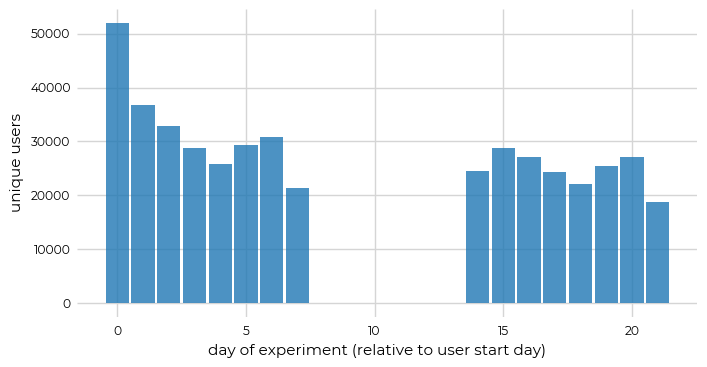
\includegraphics[width=0.9\linewidth]{figures/pioneers_per_day.png}
    \caption{Number of unique active users per day over experiment period (including intentional one-week gap.)}
    \label{fig:pioneers_per_day}
\end{figure}
%
The final dataset ultimately contained browsing data from \textasciitilde{35} million site visits and \textasciitilde{660,000} distinct domains, gathered between July 16 and August 13, 2019.
Figure~\ref{fig:domains_per_day} shows the distribution of the number of different domains per user aggregated per collection day. 
We typically see a median of 8 different domains per user per day; aggregated over the entire collection period results in a median of 34 different domains per user. 

\begin{figure}[ht]
    \centering
    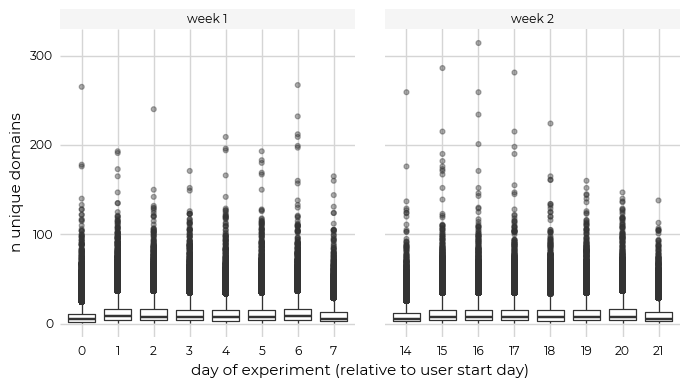
\includegraphics[width=0.9\linewidth]{figures/unique_domains_per_day.png}
    \caption{Number of unique domains visited per user per day.}
    \label{fig:domains_per_day}
\end{figure}

Restricting our domain counts to only a top-site list (details in section~\ref{ssec:selection-of-history-vector}), the median number of domains per client was 18. This is comparable to a median of 10 seen in the original paper, whose data collection methodology required use of a top-site list.
We also note that the maximum number of domains per user is 1,116. 
Although this is a lot, it is not an unrealistic amount for 14 days of browsing and is one indicator that our users were real users rather than bots or other automated tools using Firefox.

\begin{table}[hbtp]
\centering
 \begin{tabular}{@{}lll@{}}
\toprule
Min size & Max size                  & N users \\ \midrule
1        & 25                        & 21,519  \\
26       & 50                        & 11,195  \\
51       & 75                        & 6,750   \\
76       & 100                       & 4,499   \\
101      & 125                       & 2,791   \\
126      & 150                       & 1,766   \\
151      & -                    & 3,457   \\ \midrule
         & \multicolumn{1}{r}{Total} & 51,977 
\end{tabular}
\caption{Number of users by number of unique domain visits}
\label{table:profile-size-n}
\end{table}

We computed the distribution of the size of profiles across users. Table~\ref{table:profile-size-n} gives a top-level view of the relative sizes of profiles when considering all unique domains visited. 
We see a similar exponential trend as in the original work: the largest number of users have a small history size. 

We do not present the data for the number of site visits per day. 
We found some users were strong outliers with hundreds of thousands of page load events. 
We examined these manually and found that these users had one or two sites that were being hit a very large numbers of times with otherwise normal browser histories. 
We speculate that these users had browser addon(s) installed for automation of specific workflows, but were otherwise representative of normal, human browsing. 
As we represent browsing history as a boolean vector of distinct domains, thereby removing all frequency measures, we did not study this further and did not manually remove any users from the dataset.

Our data collection mechanism allowed us to capture all network requests and responses associated with site navigation events. 
Starting with complete information about the user's browsing history allows us to examine the uniqueness of browsing profiles in full depth, and make strong claims about the stability of profiles and model specific reidentification scenarios. 
Capturing all the network requests allows us to assess the potential tracking capabilities for wide range of third parties. 

Aside from the methodological differences outlined above, we note several sources of potential variation between the specific study populations. Both studies use an opt-in population, though with different methodology and flows. Our cohort provided a priori consent to longitudinal data collection, meaning a low attrition rate compared to the original work which relied on return visitors to the study website.
The original study was able to study traffic from different web browsers' users. 
They did not report on differences between browsers. However, they do mention data from 1,256 users reporting a mobile user agent.
Our WebExtension shipped to Firefox versions 67 or 68, which were release-channel versions during the study period, and ensured that the participants' browser was configured to an en-US localization, as the opt-in consent text was only available in English.
%
\subsection{Selection of a history vector}
\label{ssec:selection-of-history-vector}
The original study by Olejnik et al. required a pre-selected list of sites used to probe users' histories to see if a user had visited them. 
They sorted the list of sites by observed popularity in their dataset.
The globally ordered vector, with boolean entries for each user was then the main input to their analyses. 

As we have complete information of browsing history during the study period, we can create a history vector of the observed domains, ranked by popularity.
In our results, we label this as \textit{all observed domains}.
However, we also created a pre-defined site list for analysis.
We do this for the following reasons: (a) using a pre-defined list allows us to more closely replicate the original paper's methodology; (b) to build a category vector, we use a third-party service (see section~\ref{ssec:category-vector-generation}) and we do not want to leak user data to that service by basing our queries on user data; and (c) since history-sniffing attacks, which require a pre-defined vector, are still possible~\cite{smithBrowserHistoryRe2018}, it is relevant to perform analyses with one.

Olejnik et al's list of 6,000 popular sites was "created out of 500 most popular links from Alexa, 4,000 from the Quantcast popular websites list, lists of common government and military websites, and several custom-chosen URLs selected for their demonstration and education potential."

Pre-experiment analysis performed by Zeber~\cite{zeberTopSiteList} examined different top site lists, and led to our site list which is a hybrid of the Alexa~\cite{amazonAlexaTopSites2019} and Tranco~\cite{lepochatTrancoResearchOrientedTop2018} top 10K site lists.
We call it the \textit{Trexa} list and it is made by interleaving the sites from each and dropping duplicate entries~\cite{firefoxmachinelearningteamMozillaTrexa2020}.
The top 100 Trexa sites overlap with the 100 observed top sites in our user data by 40\%. If we expand to look at the top 10,000 sites from each list, the overlap rises to 52\%.
%
\subsection{Generation of a category vector}
\label{ssec:category-vector-generation}
%
To generate our category vector we used the WebShrinker API \cite{Webshrinker-APIs} to obtain a categorization for domains.
The entire Trexa list was run through the WebShrinker API with the Interactive Advertising Bureau categorization returned. 
The IAB taxonomy has a series of top-level and sub-level categories, with corresponding scores and confidence levels for each domain-category pair. 
We mapped each domain to its highest-rated specific subcategory, unless no such confident category existed. In that case, we substituted the most relevant higher-level category. 
If the domain was listed as "Uncategorized," we removed it from the dataset. 
Finally, we sorted from most to least observed category as we did with the all observed domains vector.
Ultimately, our categorical dataset contained 281 categories out of a total of a possible 404 offered in the IAB category standard.
The original paper used a similar categorization service called Trend Micro, which yielded 72 interest categories.
Although Trend Micro is still around today, we chose WebShrinker because the IAB categorization is in line with the threat of adtech we are interested in exploring.

\subsection{Terminology}
\label{ssec:terminology}
Throughout the paper, we use the word \textit{user} for convenience and flow, but what we are actually examining is sets of browser histories. 
The data we collected only guarantees a unique identifier for the browser. 
There may be multiple browsers per user and there may be multiple users per browser.

We refer to collections of unique user domain (or category) visits in a given time period as a \textit{profile}, as in Olejnik et al.
The profiles' underlying \textit{dataset} may be the list of all observed domain visits, Trexa domain visits, or categories. 
The \textit{size} of a profile is thus the number of unique domains or categories the profile contains.

As in the original work, and described in Section~\ref{ssec:original}, we also use the concept of a boolean \textit{profile vector}. We refer to an index of this vector as \textit{rank}; thus, a \textit{subvector-to-rank-k} describes the vector of length \textit{k} with boolean values representing whether a user has visited each of the top \textit{k} items in the dataset. Recall that the items in the vector are sorted from the most popular item in the underlying dataset to the least. 
%
%-------------------------------------------------------------------------------
\section{Replication Results}
%-------------------------------------------------------------------------------
\label{sec:replication}
%
\subsection{Web history profile uniqueness}
\label{ssec:repro-profile-uniqueness}
In Figure~\ref{fig:n_users_per_profile_size}, we compare the size of profiles when we observe all domains (as presented in Table~\ref{table:profile-size-n}), when we use the Trexa list to specify the set of domains considered, and when we use the category representation of profiles.
\begin{figure}[hb]
    \centering
    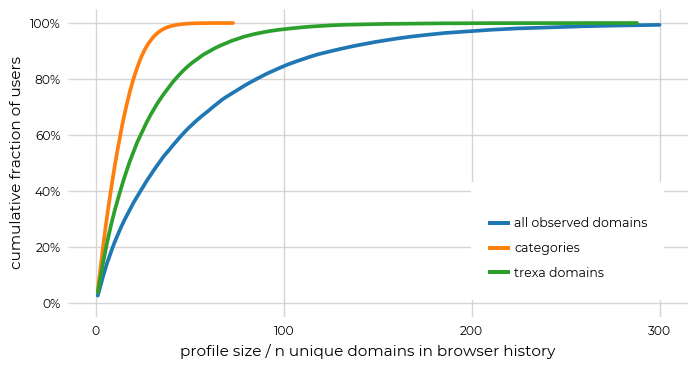
\includegraphics[width=\linewidth]{figures/fig1a_cdf.png}
    \caption{Cumulative proportion of users per profile size.}
    \label{fig:n_users_per_profile_size}
\end{figure}
%
As expected, the distribution shifts left as profiles shrink in size, relatively uniformly across the entire population.
Shifting from all domains to the Trexa list, the median profile size is reduced to 18 domains. 
Restricting to just categories, the median profile size shifts further still, to 11. 
We note that while the maximum profile size for all observed domains (1116) is much higher than its counterpart for Trexa (288) and categories (73), we observe over 99\% of all users in this plot.

In Figure~\ref{fig:profile_popularity}, we examine the distribution of prevalence of history profiles constructed from the set of all observed domains, Trexa domains, and page categories. 
The leftmost point on the x-axis represents the most common profile for each underlying dataset. 
The y-axis represents the number of users with that profile. 
In the Trexa dataset, for example, the most popular profile consists of only visits to the most popular Trexa domain, \texttt{www.google.com}, a profile which is shared by 559 users, when considering all domains in the Trexa list (brown line) and nearly 10,000 users when the domain set to build profiles from is restricted to just the top 10 sites (blue line). 
When again considering all domains in the Trexa list, the second-most popular profile consists of only visits to \texttt{www.youtube.com}, with 150 users.
Generally, the smaller the pool of users with the same profile, the more easily a specific user can be identified.
When the number of users with a particular profile reaches 1, we call that profile \textit{unique}, as it is only observed for a single user within this data collection. 
\begin{figure}[ht]
    \centering
    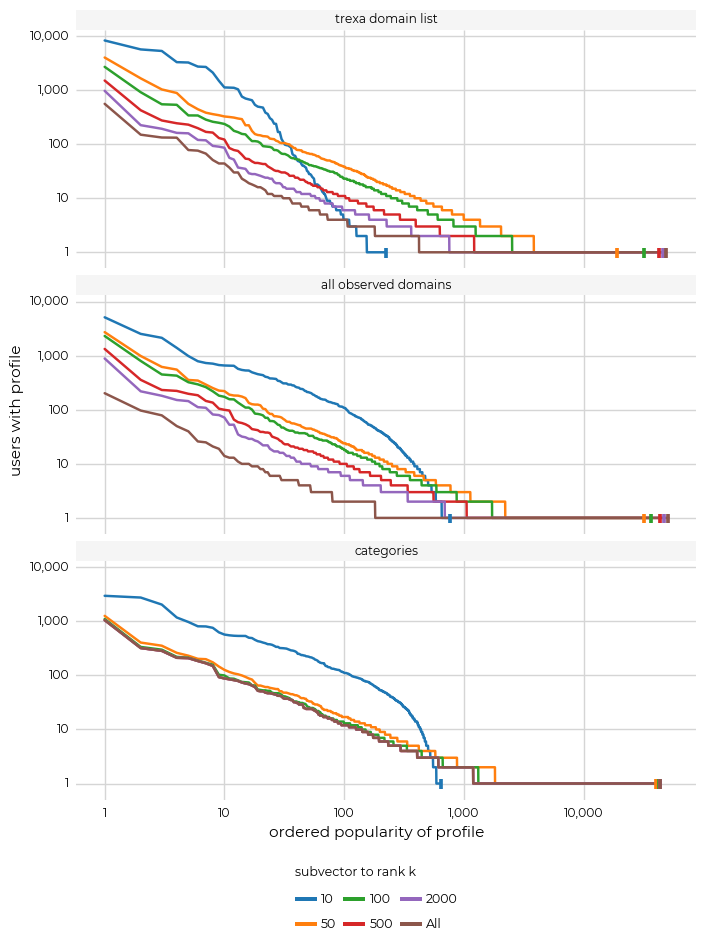
\includegraphics[width=\linewidth]{figures/4-popularity-by-k.png}
    \caption{Frequency distributions of distinct profiles ranked by popularity, across multiple subvectors of top domains.}
    \label{fig:profile_popularity}
\end{figure}
We repeated the analysis with several subvectors of the domain history, sampling up to the rank $k$ entries for various values of $k$. 
In all three datasets, $k=50$ is enough to align the slope of the line with the one generated from the entire population.
Additionally, the length of the segment at $y=1$ for each line on the chart indicates the number of profiles deemed unique.
This finding is consistent with results presented in Olejnik et al. despite the differences in the underlying datasets.

We now estimate how much identifiability is lost by only looking at a portion of a predefined domain list.
When all domains were observed, we saw 51,035 different profiles, corresponding to a 99.65\% rate of uniqueness among our users.
Restricting to visibility only the top 100 most frequently observed domains allowed us to compute 36,652 profiles (based on available histories) of which 95.31\% were unique.
Substitution of the observed domain popularity with the Trexa list led to the aggregation of 48,919 profiles of which 99.14\% were unique. 
Further constraining visibility to only the top 100 Trexa domains led to 31,810 profiles of which 92.05\% were unique.
When using the compressed data representation of just 281 categories, we still observed 43,348 profiles, of which 97.24\% were unique. 

In Figure~\ref{fig:unique_profiles_by_trexa_rank} we examine the change in proportion of unique profiles with respect to the size of the subvector more closely, looking at all values of $k$ spanning the range 1 to 250.
%
\begin{figure}[htbp]
\begin{subfigure}{.9\linewidth}
    \centering
    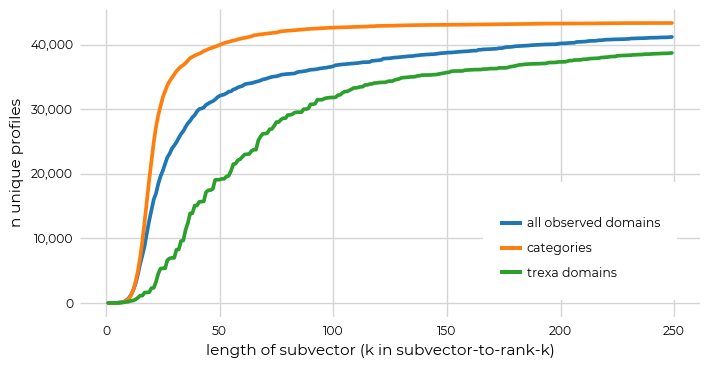
\includegraphics[width=0.9\linewidth]{figures/fig-5-a-n-unique.png}
\end{subfigure}
\begin{subfigure}{.9\linewidth}
    \centering
    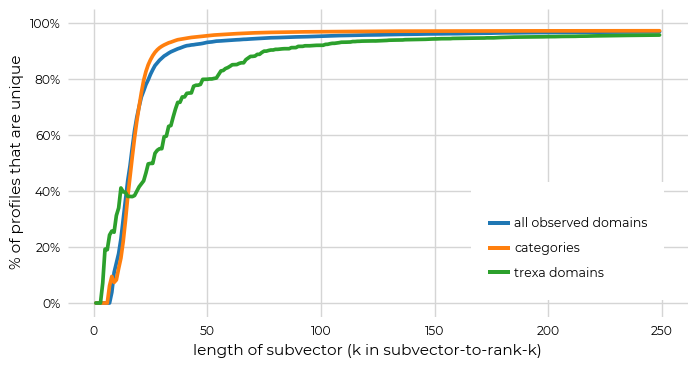
\includegraphics[width=0.9\linewidth]{figures/fig-5-b-percent.png}
\end{subfigure}
    \caption{Variation in number and proportion of unique profiles as history vector grows in size.}
    \label{fig:unique_profiles_by_trexa_rank}
\end{figure}
%
We found, unsurprisingly, that across datasets there are no unique profiles described by a profile subvector of length 1 (in the Trexa dataset, for example, there are 2 such possible profiles--users that did or did not go to \texttt{www.google.com}).
\textit{All observed domains} and \textit{categories} were ordered by the user data, describing the behavior of our users most precisely, and a large amount of these profiles quickly exhibit uniqueness.
Conversely, the ordering of the predefined Trexa domain vector does not perfectly match the population browsing data, accounting for the lack of smoothness as $k$ increases.
Although the category vector has less precision than a history vector, a category covers numerous domains; thus the category vector allows for more browsing behavior to be represented for a given $k$.
We observe that the number of distinct category profiles at the chart's elbow ($k$\textasciitilde{}30) is larger than the amount of distinct Trexa profiles by roughly a factor of 3.

Though it's straightforward to classify two profiles as distinct or not, we would like to be able to conceptualize the extent of the distance between them. Olejnik et al. used the Jaccard index to measure similarity. 
In Figure~\ref{fig:jaccard_to_self}, we use the related Jaccard distance, measured as (1 - Jaccard index), to examine the range of this distance.
%
\begin{figure}[!ht]
    \centering
    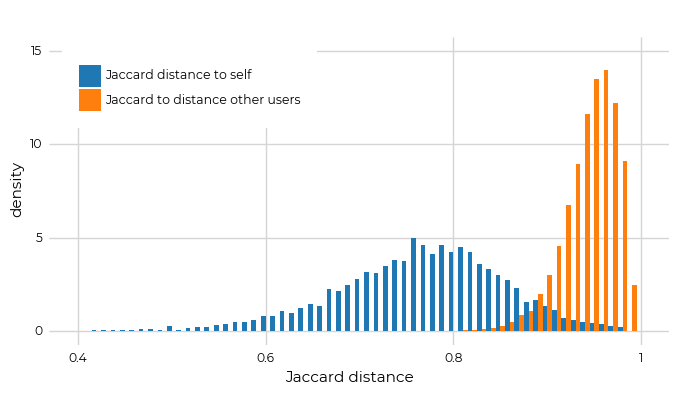
\includegraphics[width=0.9\linewidth]{figures/4-h-jaccard-to-self-1.png}
    \caption{Distribution of Jaccard distances between profiles of a single user and distinct users}
    \label{fig:jaccard_to_self}
\end{figure}
To generate the distributions in Figure~\ref{fig:jaccard_to_self}, we selected users total profile sizes of at least 50, and then split the profile into two observed activity periods. 
We then compute the Jaccard distance for the user to theirself between period 1 and period 2, and the user in period 1 to all other users in period 2.
We plot a sample of this distribution for tractability. 
Though there is overlap in the distributions, we can reasonably expect that, for a given profile, a profile from the same user has a smaller distance than one from a different user a good portion of the time. 
Repeated measures from the distribution (if we had several more time periods, for example) would only increase confidence in which distribution the measurements belongs to.

We believe that our results strengthen the original paper's claim that subsets of user data pose a potential for exploitation in user identifiability, despite differences in the underlying data.
The original manuscript observed a (likely) longer duration of history for around 7 times as many users, while we were able to collect more detailed information.
In the context of this Section, it's important to note that our smaller population increases the chances of observing a unique profile due to fewer overall profiles. 

The analysis performed above replicates the distribution of profile sizes from Olejnik et al.~Section 4.1.2, the frequency of distributions of different subvectors from Sections 4.1.3 and 4.2.3, and the distribution of Jaccard similarity from 4.1.3. In particular, we see similar trends and measurements of uniqueness, as Olejnik et al. note in Section 4.1.2, 4.1.3, and 4.2.3. 
Our similar findings regarding the uniqueness of category profiles is particularly relevant in light of the proposal for category-based targeted advertisement as a privacy safeguard put forth by some advertisement companies\cite{IAB-press-1, ICO-UK-2019}. 
In this section we did not directly address the original paper's findings related to surprisal, as in section~\ref{ssec:ext-profile-size} we use a different approach to quantifying information gain from a more detailed profile. 

\subsection{Stability of profiles}
\label{ssec:repro-stability}
The original paper examined stability of history profiles to understand the potential for browser histories to be used for tracking. 
The combination of uniqueness and stability being preconditions for reidentifiability is also discussed by G\'{o}mez-Boix et al~\cite{10.1145/3178876.3186097}.
However, the data collection method employed by the original work hindered a detailed examination of profile stability as it relied on organic return visits to the study page.  
Although over 368,000 browsing histories were collected, only a small fraction of users could be included in the stability analysis. 
They report data for \textasciitilde{1,800} returning users on day 1, dropping to \textasciitilde{400} returning users by day 7, and ~\textasciitilde{150} by day 14.
Aside from sample size considerations, two additional challenges impact the interpretation of those findings. 
Firstly, the history detection technique employed could not detect whether sites collected on first visit were revisited or first-time visits. 
Secondly, ground truth was established based on reidentifying visitors with a combination of IP Address and UserAgent, perhaps biasing the baseline data to under-represent users accessing the web from multiple locations.
In particular, accurate estimation of site revisitation rates is vital to estimating the possibility of reidentifiability.

Our methodology gathered two weeks of browsing data from all our users.  
Although we do see a drop in the number of users over the course of the study as visible in Figure~\ref{fig:pioneers_per_day}, we have two weeks of browsing data from tens of thousands of users allowing us to model the reidentification of users based on browsing history.
Due to the fundamental differences between the datasets, we have not attempted to replicate the original paper's stability analysis. 
Instead, we extend the original work and model reidentifiability as outlined in Section~\ref{sec:extension}. 
We note here that our work supports the original finding that browser history profiles are stable.
%
\subsection{Third parties}
\label{ssec:repro-third-parties}
As our data collection included all requests and responses, we are able to see all third parties that users were exposed to. 
We find the results from the original paper are not only reproducible, but are stronger today with Google (Alphabet) and Facebook observing large portions of the web. 
Presentation of our third-party analyses is available in the extension section~\ref{ssec:ext-third-parties} where we examine the theoretical reidentifiability of the top third parties our participants were exposed to.
%
%-------------------------------------------------------------------------------
\section{Reidentification rates extension}
%-------------------------------------------------------------------------------
\label{sec:extension}
As previewed in Sections~\ref{ssec:repro-stability} and~\ref{ssec:repro-third-parties}, we wish to expand on the work illuminating the privacy risk that Olejnik et al.~\cite{olejnikWhyJohnnyCan2012} describe. We do so by directly modeling the reidentifiability of users based on their browsing history. As we move into this section, recall that while we continue to talk about profiles, as described in Section~\ref{ssec:terminology}, we now consider each user separately. If two different users have the same history profile, they appear as two identical rows in our dataset and the matching process, as explained in~\ref{ssec:ext-metric}, will randomly select between those two users. For all the analyses presented, period 1 and period 2 are the two weeks of browsing data separated by a week. 
%
\subsection{Reidentifiability metric}
\label{ssec:ext-metric}
As motivated by the distributions in Figure~\ref{fig:jaccard_to_self}, we define a model for attempting to reidentify a user between observation sessions.
For each user, we compute the Jaccard distance between the user's period 1 profile vector and all profile vectors in week 2. The period 2 browsing history vector with the lowest Jaccard distance to the profile of interest is considered the most likely match. (Note: We did not build special handling for ties. We used the pandas \texttt{idxmin} function which returns the "index of first occurrence of minimum over requested axis". As the identifier is a randomly generated alpha numeric code, we do not believe this introduced bias into our results.)
We then evaluate the match and a user is considered \textit{reidentified} if the correct identification was made. The reidentifiability rate is thus the percentage of all users in a specified pool who are reidentified in this manner. 

Though the minimum Jaccard distance is a very simplistic metric to use for this analysis, we chose it for a number of reasons. 
Firstly, it directly follows from the examination of Jaccard distances between profiles in the original paper. 
Secondly, it is easy to interpret: this metric picks the period 2 vector with the most overlap between both sets.
Lastly, and perhaps most importantly, building a reidentifiability engine is a complex task with several domain-specific algorithmic choices to consider. 
Subtler distance metrics, multinomial data (modeling the frequency of domain visits), and more detailed browsing metadata (time of browsing, for example, or more privacy-invasive features that could be collected in the wild) could all improve our matching algorithm significantly.
However, our goal is to take the next logical step beyond the analysis of profile uniqueness to understand whether that uniqueness implies a level of reidentifiability worth exploring. 
Because of possible model improvements previously mentioned, we can safely consider the results we obtain to be an underestimate of analagous methods potentially used in industry. 

We note that throughout the following analyses we split users into groups by their overall profile size (the number of distinct domains in their total browsing history). It is done once to sub-divide the population. It is not recomputed for each type of analysis and serves solely as a way to stratify the population so that inter-group comparisons are valid.
%
\subsection{Baseline reidentifiability}
\label{ssec:ext-basic-rejoinability}
%
We start our analysis by looking at the reidentifiability of all users with more than 50 distinct domains in their complete browsing history.
We start with this number as a trade-off between two factors: (a) as we will show later in Section~\ref{ssec:ext-profile-size}, reidentifiability increases as the number of unique domains in a user's profile increases, and (b) as shown in Figure~\ref{fig:n_users_per_profile_size}, the smaller the minimum profile size we consider, the larger the pool of users we have. 
Restricting to a minimum profile size of 50 domains results in 19,263 users, 37\% of the total in our dataset. This number is tractable for computation and yields significant reidentifiability rates.

With the data split into two profile vectors for the distinct time periods, we compute the reidentifiability metric at various subvectors of rank k.  
Once we had the vector of evaluated reidentifications (True/False for each user), we resampled it 10,000 times to find the bootstrapped confidence interval for the rate of reidentifiability. Figure~\ref{fig:rejoin-sall50plus} shows these results for both the set of all observed domains and the Trexa list domains.
%
\begin{figure}[htbp]
    \centering
    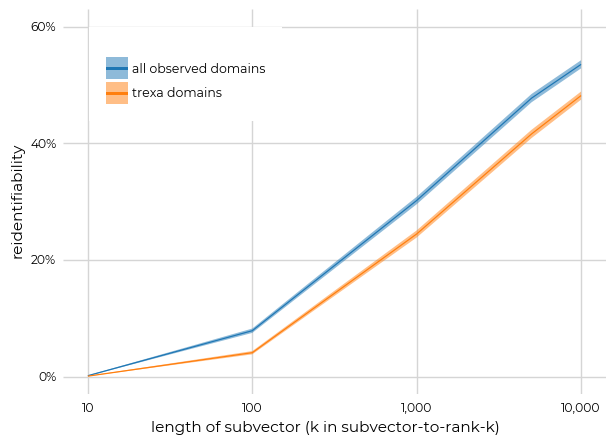
\includegraphics[width=0.9\linewidth]{figures/4-c2-2-rejoinability-by-rank-trexa-pioneer-50plus.png}
    \caption{Reidentifiability over two domain lists for 19,263 users with a profile size over 50}
    \label{fig:rejoin-sall50plus}
\end{figure}
%
The first thing we can observe from Figure~\ref{fig:rejoin-sall50plus} is the tightness of the 95\% confidence intervals due to the population size. The relative width of these intervals can be contrasted with those in Figure~\ref{fig:rejoin-by-rank-by-group}.  
Second, we observe that, unsurprisingly, the more domains  included in the computation, the higher the reidentifiability rates.
This makes intuitive sense: as we increase the rank of the subvector, we include both less-common sites and combinations of sites that are more likely to be specific to a particular user profile.
Interestingly, we note that although a subvector truncated at rank 100 leads to a high proportion of unique profiles (92-95\%), the reidentifiability rates are below 10\% for both datasets. However, when we include the subvector to rank 10,000, reidentifiability rates grow to \textasciitilde{}50\%. 
Additionally, the difference in reidentifiability across the two datasets is smaller than we may have expected given the relatively large difference between the two lists.

The upward trend in reidentifiability as the length of the subvector increases makes sense, but we must also consider the effect of stability of browsing activity. The more consistent a history is, the easier it is to reidentify with smaller amounts of data. For example, consider a light internet user that regularly goes to the same 5 websites, compared with a heavy internet user that spends many hours a day browsing but rarely the same domains.
Understanding types of users, and patterns of browsing behavior, is a relevant problem but outside the scope of this paper.
%
\subsection{Modeling scaling effects}
\label{ssec:ext-scalability}
%
Another concern for a real-world implementation is the scale of the user pool. 
In a pool of a single user, reidentifiability is necessarily 100\%.
As the pool of potential candidates grows, the signal must be increasingly specific in order to correctly match two user profiles.

Measuring scalability is ideally done by collecting the browsing data of millions of people. Unfortunately, this method is infeasible within the limits of our research. 
Additionally, this type of collection involves privacy risk, although we note that this practice is commonly employed by companies engaged in cross-site tracking activity.

To explore scalability with the data we have available to us, we perform a Monte Carlo simulation with the subset of users with a profile size over 50. We sample between 1 and the max number of users 55,000 times without replacement, and calculate the subvector of observed domains at rank 10,000 for each user's profile. The sampling volumes were designed to give good coverage over the log space of n users. The results are shown in Figure~\ref{fig:rejoin-scaling}.
%
\begin{figure}[htbp]
%\captionsetup[subfigure]{justification=centering}
\begin{subfigure}{.9\linewidth}
    \centering
    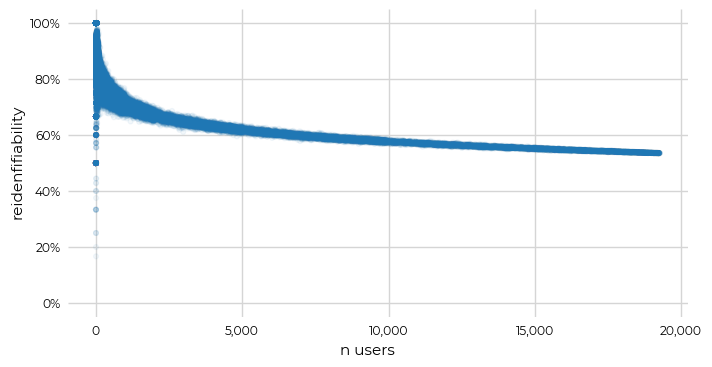
\includegraphics[width=0.9\linewidth]{figures/4-f-scalability-linear.png}
    %\caption{Linear scaling of n users}
    %\label{subfig:rejoin-lin}
\end{subfigure}
\begin{subfigure}{.9\linewidth}
    \centering
    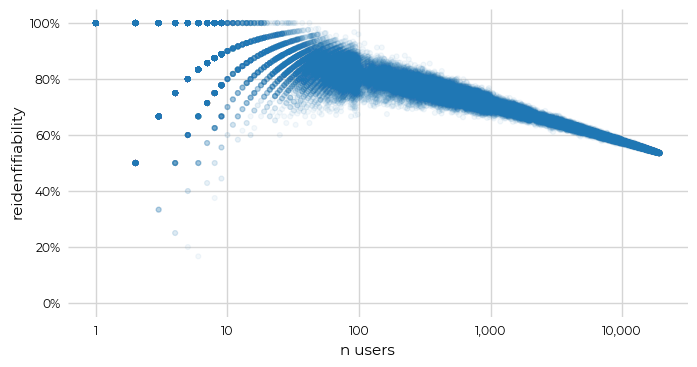
\includegraphics[width=0.9\linewidth]{figures/4-f-scalability-log.png}
    %\caption{Log\textsubscript{10} scaling of n users}
    %\label{subfig:rejoin-log}
\end{subfigure}
\caption{How reidentifiability scales with the number of users in a pool. Simulation for all users with profile size over 50. Linear axis (above) and log axis (below).}
\label{fig:rejoin-scaling}
\end{figure}
%
The log scale in the lower plot causes the striations in reidentifiability on the left of the lower plot, which are an artifact of the limited value space for reidentifiability with small n ($n=1$ has a reidentifiability rate set of $\{1\}$, $n=2$ has $\{0, 0.5, 1\}$, etc.).

The top chart suggests that the reidentifiability rate reaches an asymptote, bolstered by the linearity on the log scale chart. 
However, it does not feel prudent to say that the trend is certain for millions of users. 
We leave this analysis to future research. 
We can, however, make claims about the effects of reducing the pool of users. 
Roughly speaking, a 10-fold reduction in the number of users increases reidentifiability by 10\%. 
This is relevant as we now turn to looking at how reidentifiability risk increases as the number of domains in a profile increases.
%
\subsection{Effect of profile size}
\label{ssec:ext-profile-size}
%
Understanding the effect of profile size on reidentifiability can illuminate certain threat models.
For example, if only a modest threshold for profile size is needed, can a short private browsing mode session provide enough activity to allow reindentifiability, despite the precautions taken?
 
To understand the effect of profile size alone it is important to constrain our data in new ways. We divide the data into 7 groups with profile sizes as shown in Table~\ref{table:profile-size-n}.
We selected buckets that added 25 domains at a time so that the smallest bucket, by number of users, still had a meaningful 1,766 users.
As shown in Section~\ref{ssec:ext-scalability}, the number of users in a reidentifiability pool affects the reidentifiability rate, so we constructed our buckets to all be the same size in order to isolate the effect of profile size.
Specifically, we sampled without replacement 1,766 users from each bucket.
We then computed the reidentifiability rate and the bootstrapped confidence interval (n=10,000) at various subvector lengths as done in Section~\ref{ssec:ext-basic-rejoinability}. 
We repeated this process with a second downsampled set to validate that the downsampling did not overly bias the outcome.
The results are presented for the first downsampled set in Figure~\ref{fig:rejoin-by-rank-by-group}.
%
\begin{figure}[htbp]
    \centering
    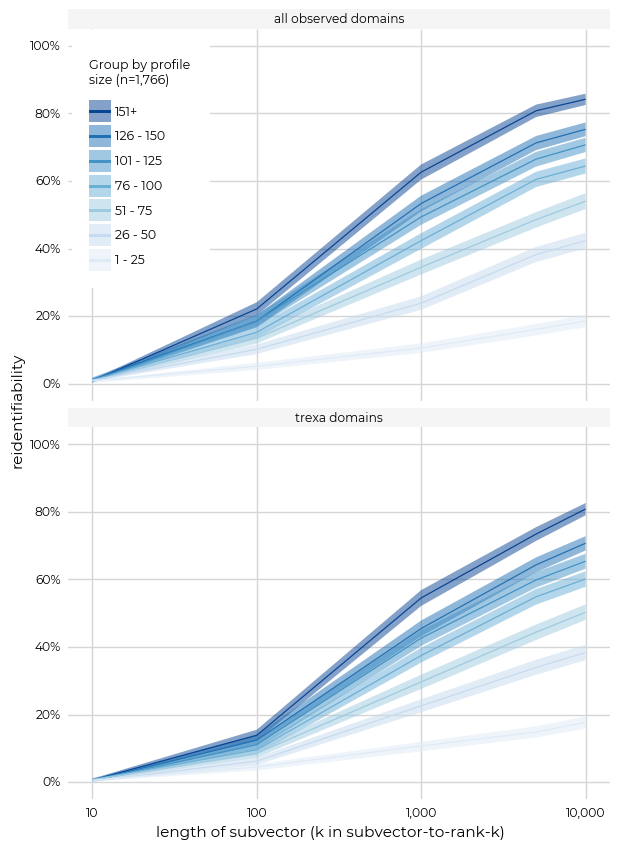
\includegraphics[width=0.9\linewidth]{figures/4-c2-1-rejoinability-by-rank-trexa-pioneer-subgroups.png}
    \caption{Reidentifiability across varying profile sizes}
    \label{fig:rejoin-by-rank-by-group}
\end{figure}
%
As Figure~\ref{fig:rejoin-by-rank-by-group} shows, reidentifiability increases as profile size increases up to \textasciitilde{}80\% for users with over 150 distinct domains in their profile.
We note the wider 95\% confidence intervals compared to those in Figure~\ref{fig:rejoin-sall50plus}, which is expected with the smaller sample in each group.
If we look at the reidentifiability rate for the group with profile size 51-75, we see it is a little higher than that shown for the 50 plus group shown earlier in Figure~\ref{fig:rejoin-sall50plus}. 
There are two competing forces here: (1) the smaller pool of users in in this analysis drives higher reidentifiability, but (2) the cap on the size of the profile at 75, as opposed to no cap in Figure~\ref{fig:rejoin-sall50plus}, limits reidentifiability.

We observe that as the size of bucket increases, the reidentifiability rate increases. 
However, the increase diminishes with each additional increase in profile size.
At rank 10,000 the reidentifiability rate jumps \textasciitilde{}20\% when the profile size increases from 1-25 to 26-50. 
However, the increase is less than 5\% when going from 101-125 to 126-150.
The additional separation seen by the largest group (151+) is an artifact of that bucket incorporating some much larger profiles.

As seen in section~\ref{ssec:ext-metric}, Trexa reidentifiability rates are not dramatically different despite the difference in these domain lists. 
This similarity highlights the viability of history sniffing attacks as tracking vectors, event though we found Trexa to only have 52\% overlap with observed user top sites.
In Figure~\ref{fig:rejoin-by-rank-by-group}, we note the "contraction" in the reidentifiability rates at k=100, which is consistent with our observation that the top 100 Trexa list overlaps with the observed browsing history less than it does for the top 10,000.
%
\subsection{Reidentifiability with category profiles}
\label{ssec:ext-categories}
Using the category profiles from Section~\ref{ssec:repro-profile-uniqueness} we computed reidentifiability rates with the full-length 281 category vector for the same buckets of users as Section~\ref{ssec:ext-profile-size}. The rates are shown below in Table~\ref{table:cat-reidentify-rate}.
%
\begin{table}[htbp]
\centering
\begin{tabular}{ll}
\hline
Profile size & \begin{tabular}[c]{@{}l@{}}Category-based reidentifiability rate\\ (95\% confidence interval)\end{tabular} \\ \hline
1 - 25       & 5.8\% (4.8\% - 6.9\%)                                                                   \\
26 - 50      & 10.0\% (8.6\% - 11.4\%)                                                                  \\
51 - 75      & 14.3\% (12.7\% - 16.0\%)                                                                \\
76 - 100     & 15.7\% (14.0\% - 17.4\%)                                                                \\
101 - 125    & 16.5\% (14.8\% - 18.3\%)                                                                \\
126 - 150    & 19.1\% (17.3\% - 21.0\%)                                                                \\
151+         & 23.3\% (21.3\% - 25.3\%)                                                                \\ \hline
51+          & 8.1\% (7.7\% - 8.5\%)                                                                   \\
\end{tabular}
\caption{Reidentifiability rate over category profiles}
\label{table:cat-reidentify-rate}
\end{table}
%
The reidentifiability for categories is limited but non-zero. 
The rates are consistent with domain vectors of a similar length.
We note, as in Section~\ref{ssec:ext-basic-rejoinability}, that although this small number of categories is sufficient to yield a large number of distinct profiles, it does not yield high reidentification using our metric.
As noted by Olejnik et al., the category analysis is an obvious candidate for a multinomial approach, using the frequency of category visits instead of the binary vector. 
However, as outlined in Section~\ref{ssec:ext-metric}, we chose to stick to a single reidentifiability metric. 
We look forward to further work examining the impact of a more sophisticated model.
%
\subsection{Third-party reidentifiability}
\label{ssec:ext-third-parties}
The original paper~\cite{olejnikWhyJohnnyCan2012} constrained an examination of third parties to the subset of domains on which third-party scripts from Google or Facebook were observed.
Our data collection included all request and response data during the data collection period, allowing a direct identification of all third parties present on a site during a user's visit.
However, the very definition of a third-party relationship at the domain level has become increasingly complex. 
On the web today, individual actors, such as Oracle or Wikipedia, operate their services on multiple domains.
This presents three problems: (1) The reach of one third-party domain does not accurately characterize an entity's reach; (2) an entity using a separate domain to serve their own content on their main site, for example media on wikipedia.org is hosted by wikimedia.org will be identified as a third party; and (3) an entity may have a corporate or operational structure such that it has insight into data collection performed by other companies, through common ownership or data exchange agreements.
To overcome these challenges we use the webXray domain list~\cite{Libery-Web-xray, TimlibWebXrayDomain} which connects domains with corporate entities and codifies corporate structures.
For consistency we associate all domains with the highest level parent entity in the webXray dataset.
So, for example, we capture the third-party reach of Alphabet, Google's parent company.

We mark all requests with the parent entity they are associated with. If the parent entities of the request and the navigation domain differ, the request marked as third party.
We measured the most prevalent third parties with two metrics: the number of first parties a third-party entity is present on, and the number of users who were exposed to that third party.
We took the union of the top 50 by each metric to create a list of 61 prevalent third parties. 
To preserve privacy, we filtered this list to only contain third-party entities to which more than 5,000 users had been exposed.
This step resulted in the removal of 1 third party, leaving a list of 60 third-party entities to analyze.

We started with the top 10,000 observed domains and reduced it to the set visible by the third-party entity.
This limits the set of domains we are considering compared to the full reach of the entities. 
However, it also makes the result directly comparable with Figure~\ref{fig:rejoin-by-rank-by-group}, along with being more computationally tractable.
The results are presented in Figure~\ref{fig:rejoin-webiverses} for three groups of users: the complete set of 19,263 users with over 50 domains in their complete profile shown in Figure~\ref{fig:rejoin-sall50plus}, the set of 1,766 users with a profile size over 150 domains shown in Figure~\ref{fig:rejoin-by-rank-by-group}, and a randomly selected set of 1,766 users from those with a profile size over 50. 
This last set provides a link between the other two, enabling direct comparisons for both number of users and profile size.
%
\begin{figure}[ht]
    \centering
    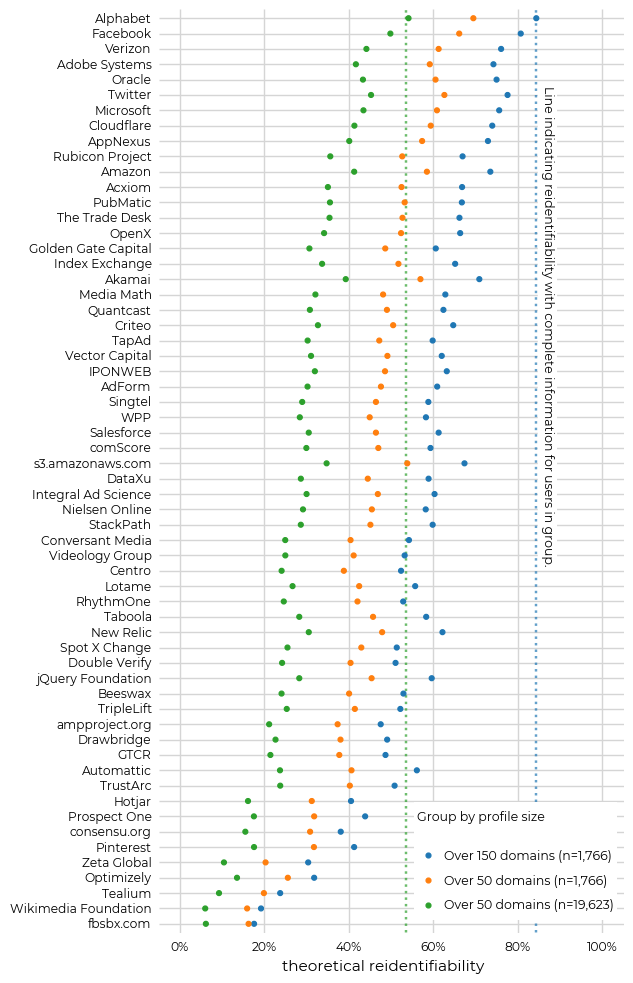
\includegraphics[width=0.9\linewidth]{figures/4-e2-webiverses.png}
    \caption{Theoretical third-party reidentifiability rates}
    \label{fig:rejoin-webiverses}
\end{figure}
%
Figure~\ref{fig:rejoin-webiverses} provides a number of important insights. 
Firstly, we observe that the steps between the three user groups are consistent across third parties, and are consistent with our results in earlier sections. 
We note that the results are presented as theoretical reidentifiability rate in order to highlight that we are not claiming the entities presented are all performing this kind of an attack.
That said, TapAd and Drawbridge, two leading probabilistic trackers~\cite{biltonCrossdeviceTrackingExplained2015, brookmanCrossDeviceTrackingMeasurement2017}, are present in our top third-party list with a theoretical reidentifiability rate of approximately half the rate we obtained with complete information.
Alphabet and Facebook, the two entities studied in the original paper, have close to our computed maximum, which is significantly higher than what the original authors found relative to their core metric of uniqueness. 
We summarize third parties as being highly prevalent and with the potential for deep visibility into browsing activity; that potential for surveillance is not in and of itself proof thereof.
%------------------------------------------------------------------------------
\section{Discussion}
%------------------------------------------------------------------------------
\label{sec:discussion}
%
Our findings on profile uniqueness replicate those of Olejnik et al.~\cite{olejnikWhyJohnnyCan2012} and our work on reidentifiability provides robust evidence for the viability of browser profiles as a tracking identifier.
Interpretation of these extended findings as it pertains to third parties requires a nuanced examination of the underlying data.
Notably, Wikimedia Foundation was observed on 395 of the top 10,000 first-party domains.
This is low in relation to Alphabet (parent company of Google) at 9,823, and Facebook at 7,348, and the numerous companies from Verizon to TrustArc with a presence on 2,000 - 5,500 of the top 10,000 first-party domains. 
Nonetheless, 395 first-party domains could still be considered surprising for a non-profit organization likely not engaging in data surveillance activities.
The surprisingly large presence of Wikimedia is at least partially due to user-generated content, where individuals make use of web platforms to share content via third-party links.
This observation raises important questions about methodological due diligence when interpreting third-party relationships for the purpose of privacy and security research.

To use a history profile as a tracking vector, one must first be created. 
This means an entity requires some visibility into browsing behaviour via another tracking identifier to enable data collection over a time period, or they must perform a history sniffing attack. 
In some jurisdictions, history sniffing is likely illegal~\cite{bellovinHistorySniffing2012} and in the US led to the FTC bringing charges against a company~\cite{FTCApprovesFinal2013}.
This type of attack is very hard for users to prevent, and responsibility rests with researchers and browser vendors to remain vigilant in monitoring vulnerabilities such as those disclosed by Smith et al.~\cite{smithBrowserHistoryRe2018} to protect global web users.

The most prevalent tracking identifier is a browser cookie; however, as awareness of cookies has increased so have user protections.
Currently, tracking protections built into Firefox, Edge, Safari, and Brave attempt to limit or block tracking content. 
Protections are not complete for a variety of reasons; often compromises are made to avoid unexpected errors in the way web pages are loaded as web browsers must correctly display web content while selectively blocking content designed by web developers.
In January 2020, Chrome made headlines announcing that they will phase out third-party cookies~\cite{BuildingMorePrivatea}.
The W3C Privacy Community Group, with members from all major browsers and a wide-range of stakeholders, proposes going much further with Client-Side Storage Partitioning (CSSP)~\cite{w3cprivacycommunitygroupClientSideStoragePartitioning}.
CSSP will link access to a wide-range of browser features to a first-party domain.
In a simple case, if \texttt{tracker.example} sets a cookie on \texttt{a.example}, on \texttt{b.example}, \texttt{tracker.example} will not see that cookie.
In principle, CSSP will make the web profoundly more private than it is today, and its scope is far beyond cross-site cookies.
Versions of this type of protection can be seen in Safari ~\cite{wilanderFullThirdPartyCookie2020,wilanderIntroducingStorageAccess2018}, Firefox Nightly~\cite{MozillaAddsDynamic}, Tor Browser~\cite{DesignImplementationTora}, and Brave~\cite{braveOKGoogleDon2020} as of April 2020.

Even if traditional stateful tracking is addressed, IP address tracking and fingerprinting are a real concern as ongoing privacy threats that can work in concert with browser history tracking.
We point readers to Mishra et al.'s~\cite{mishra:hal-02435622} discussion on IP address tracking and possible mitigations.
They observed IP addresses to be static for as long as a \textit{month} at a time, and while not a perfect tracker, IP addresses are trivial to collect.
Our reidentifiability metric tracked users from one week to the next using only one week of web browsing history to build a profile (see Section \ref{sec:extension}).
Technical solutions such as VPNs and Tor can offer imperfect protection~\cite{mishra:hal-02435622, padmanabhanReasonsDynamicAddresses2016}, as can efforts on behalf of Internet service providers to refresh users' IP addresses more frequently.

There is a growing technical emphasis on efforts to mitigate browser fingerprinting.
G\'{o}mez-Boix et al.~\cite{10.1145/3178876.3186097} found that browser fingerprints are not perfect identifiers, but did observe that 95\% of desktop users had fingerprints that matched 100 or fewer other users.
Presuming that device-specific properties (screen size, graphics stack) are not correlated with browsing history, then fingerprinting offers a mechanism to greatly narrow a pool of users in which to associate browsing histories.
As we have shown, the smaller the pool of users under consideration, the higher the reidentifiability rates achievable with browsing history alone (see Section \ref{ssec:ext-scalability}).

We are encouraged that fingerprintability is a consideration in web specifications~\cite{MitigatingBrowserFingerprintingb}, but a significant amount of work remains if we are to prevent fingerprinting and we hope researchers and browser vendors will push aggressively on anti-fingerprinting measures.
%-----------------------------------------------------------------------------
\subsection{User-facing recommendations}
\label{sec:recs}
%-----------------------------------------------------------------------------
Until the state of the web has improved, the onus of ensuring privacy often falls on the user.
However, evidence suggests that general audiences are not aware that privacy protection tools exist, let alone understand their function or the threats they protect against~\cite{ChanceryUserPerceptions}.
Additionally, Fagan et al.~\cite{faganWhyDoTheyDo} describe the trade-off between convenience and security that often results in non-compliance with security measures unless the risk can be understood and evaluated.

Currently, users can limit their exposure to third-party tracking by opting into tools such as privacy addons~\cite{frankenWhoLeftOpen2018,mathurCharacterizingUseBrowserBased2018,merzdovnikBlockMeIf2017}, containers~\cite{mozillaMultiAccountContainers}, and by modifying their browser settings to emphasize existing privacy features that may result in a diminished browsing experience. 
Blocking fingerprinting via the Disconnect list in Edge and Firefox offers users protection, but relies on a blocklist of known trackers.
Privacy addons offer fingerprinting protections through lists such as EasyList and EasyPrivacy~\cite{EasyListOverview}, or a fine-grained control over locally curated exclusion lists, which require substantial effort by users to maintain.
Tor Browser includes changes to reduce the entropy of the browser by normalizing the return values of various APIs~\cite{DesignImplementationTora}. 
This functionality is also available in Firefox behind the \texttt{privacy.resistFingerprinting} configuration flag, but introduces compatibility issues with some websites.
Chrome's Privacy Sandbox project~\cite{PrivacySandboxChromium} proposes the concept of a privacy budget~\cite{lasseyBslasseyPrivacybudget2020} that only allows a certain amount of entropy to accumulate, along with reducing entropy and removing fingerprinting surfaces. 

As the existence of these tools alone is not enough to prevent a tracking threat, well-researched user experience practices should be considered in order to increase their adoption and make their usage more seamless while mitigating drawbacks.
Mathur et al.~\cite{MathurPreventOnlineTracking} propose that browsers should automatically provide comprehensive protection in particularly sensitive contexts such as private browsing mode.
We did not collect data when a private browsing mode session was active, and so cannot validate our threat model in this context. 
However, the potentially sensitive nature of private browsing indicates that the need to avoid tracking may overpower the need to avoid breakage or inconvenience the user.
Developers of products with private browsing modes should not only encourage their use when appropriate, but enforce short, task-focused sessions to reduce the number and diversity of domains visited, potentially by purging a session when a threshold has been reached or by encouraging good user habits via messaging, suggestions, or other interaction design.

Our research leaves a number of open questions that must be considered in the face of designing user interventions for browser history tracking. 
In particular, there are questions about how to educate users and offer meaningful privacy protections against the kind of complex and abstract threat model we outline.
The many tools that currently exist to preserve privacy should be encouraged within the context of a well-explained, specific threat to empower users to opt in to these tools on an ongoing basis.
%
\subsection{Limitations and future work}
\label{sec:limitations}
%
It is our hope that these findings will be appropriately interpreted despite, and in context of, limitations to the data collection methodology, reidentifiability metric, and the analysis of third-party relationships.
As with any opt-in data collection, our data represents a biased sample. 
We cannot know the exact effect of this bias; however, we suggest that our sample may exhibit greater homogeneity than we expect from the overall internet-connected population.
This may have resulted in an underestimation of the ease with which participants can be reidentified based on browsing histories.

We believe our replication provides an important and complementary extension to the original, as we were able to directly study reidentification threats.
Although we have similar concerns regarding the feasibility with which such tracking threats can be scaled to billions of web users, our discussion in Section \ref{sec:discussion} provides anecdotal evidence that it is feasible to combine independent tracking vectors, which would can dramatically reduce the required scale for viability.

Our model leverages a very basic metric to demonstrate reidentifiability.
It was our intention to focus on the question of moving from uniqueness of profiles to a baseline reidentifiability rate. 
As described in section~\ref{ssec:ext-metric}, there is a multitude of more advanced techniques available. 
For example, Banse et al.~\cite{Banse_2012} achieved an 88.2\% reidentification rate among 2,100 users based on daily browsing data using a Naive Bayes classifier and cosine distances.
Perhaps more importantly, companies engaged in this kind of activity have access to the full range of tracking data: IP addresses, cookie-based identifiers, identifiers from cookie-syncing, click attribution identifiers, browser fingerprints, and user-generated identifiers such as social media handles or email addresses used for logins.
We do not want to over-speculate on the relative impact of these factors, but we do believe that the approach presented in this work, in spite of the above caveats, is conservative when it comes to the potential for using browser history as a tracking profile.

We would like to highlight a core limitation of our approach to measuring third parties at the entity level and why we believe it is still preferable to other strategies for discerning relationships between web resources. 
This limitation is exemplified by the presence of \texttt{fbsbx.com}, a Facebook-owned domain, on our top third-party list.
This domain was observed on only 351 of the top 10,000 first-party domains, but its inclusion in our list was based on its visibility to users as a third party. 
This was driven by the fact that the webXray dataset does not currently associate \texttt{fbsbx.com} as being part of the Facebook entity and so requests to \texttt{fbsbx.com} were marked as third-party in nature when they originated from visits to \texttt{facebook.com} and other popular Facebook owned first-party sites.
It is difficult to know how many times this has happened during our data analysis; we consider the implications of this finding and caveat our results accordingly. 
If a domain is not associated with an entity in the webXray list it has the following possible effects: (1) The presence / traffic of that domain in a third-party context is not correctly associated with the entity, thereby lowering the power of the third-party in our reidentifiability analysis, and (2) Missing the third-party relationship with a domain only affects the reidentifiability analysis by the number of first-party domains the third party has been misidentified on. 
In the case of Facebook not being linked with \texttt{fbsbx.com}, we may have incorrectly labeled it as having a third-party relationship with Facebook domains such as \texttt{facebook.com}, \texttt{instagram.com}, \texttt{whatsapp.com}. 
The fact that \texttt{fbsbx.com} is not correctly associated with Facebook has lowered the Facebook reidentifiability rate by up to 350 domains, but it has raised the \texttt{fbsbx.com} domain rate by only a handful of domains. We are comfortable with this trade-off despite the fact that using an entity list introduces a dependency on its accuracy and completeness. 
Correctly characterising a third-party relationship in the context of web research is, itself an immensely complex undertaking and there is an abundance of future work to be done in this space.  

Finally, we did not find all profiles to be unique or reidentifiable. Future work should leverage the common traits in these non-unique profiles in order to inform strategies for privacy tools and education development.
%-------------------------------------------------------------------------------
\section{Conclusion}
\label{sec:conclusions}
%-------------------------------------------------------------------------------
In summary, we set out to replicate and expand upon the ideas put forth in Olejnik et al.'s 2012 paper \textit{Why Johnny Can't Browse in Peace: On the Uniqueness of Web Browsing History Patterns}. 
The original paper observed a set of \textasciitilde{}400,000 web history profiles, of which 94\% were unique. 
Our set of 48,103 distinct browsing profiles, of which 99\% are unique, followed similar distributions as the original.
Likewise, these patterns held when we used a public top-site list and category mappings to restrict visibility into the number of domains considered, mimicking the methodology of the original work. 

Olejnik et al. found evidence for profile stability among a small pool of returning users.
We extend this work and modeled reidentifiability directly for nearly 20,000 users. We reidentify users from two separate weeks of browsing history, and examine the effect of profile size, and how reidentifiability scales with the number of users under consideration.
Our reidentifiability rates in a pool of 1,766 were below 10\% for 100 sites despite a >90\% profile uniqueness across datasets, but increased to \textasciitilde{80\%} when we consider 10,000 sites. 
Finally, while Olejnik et al. show somewhat lower uniqueness levels for profiles of pages tracked by Google and Facebook, we show theoretical reidentifiability rates for some third-party entities nearly as high as those we achieve with complete knowledge of all visited domains. 
%
%-------------------------------------------------------------------------------
\section*{Acknowledgments}
%-------------------------------------------------------------------------------
We extend a sincere thanks to Olejnik, Castelluccia, and Janc, the authors of the original manuscript~\cite{olejnikWhyJohnnyCan2012}, for providing the inspiration for this work and their contributions to the advancement of privacy technology. In particular, we thank Lukasz Olejnik for his communication and collegiality throughout the duration of this research.

The authors also thank the numerous individuals who participated in reviewing both the codebase enabling this work, and earlier versions of the manuscript. Thanks to David Zeber, Fred Wolls\'{e}n, and Victor Ng on the Firefox Machine Learning team for supporting this research line as well as Mozilla's data pipeline engineering, data operations, and quality assurance teams.

Finally, the authors would like to thank all of the Firefox users who continue to trust us with their private data through their voluntary enrollment into experimental initiatives.
%------------------------------------------------------------------------------
\bibliographystyle{plain}
\bibliography{bibliography.bib}
%------------------------------------------------------------------------------
\end{document}